%%%%%%%%%%%%%%%%%%%%%%%%%%%%%%%%%%%%%%%%%%%%%%%%%%%%%%%%%%%%%%%%%%%%%%%%%%%%%%%%%%%%%%%%%%%%%%%%%%%%%%%%%%
%Write by:ShuwenHe
%Date:20230613
%%%%%%%%%%%%%%%%%%%%%%%%%%%%%%%%%%%%%%%%%%%%%%%%%%%%%%%%%%%%%%%%%%%%%%%%%%%%%%%%%%%%%%%%%%%%%%%%%%%%%%%%%%

%%%%%%%%%%%%%%%%%%%%%%%%%%%%%%%%%%%%%%%%%%%%%%%%%%%%%%%%%%%%%%%%%%%%%%%%%%%%%%%%%%%%%%%%%%%%%%%%%%%%%%%%%%
\documentclass[12pt,twiside,a4paper]{ctexbook}
\usepackage[centertags]{amsmath}
\usepackage{amsfonts}
\usepackage{amsthm}
\usepackage{newlfont}
\usepackage{makeidx}
\usepackage{tabularx}
\usepackage{wasysym}
\usepackage{geometry} 
\usepackage{graphics}
\usepackage{slashbox} 
\usepackage{fancyhdr} 
\usepackage{ulem} %下划线、删除线、波浪线
\usepackage[pdftex]{graphicx}
\usepackage{epstopdf}
\usepackage{cite}
\usepackage{listings}
\usepackage{tocbibind}
\usepackage[numbers,sort&compress]{natbib}

\setlength\parskip{\baselineskip}
\setcounter{tocdepth}{8} % 生成目录层级
\setcounter{secnumdepth}{4}
\renewcommand\thesection{\arabic{section}}
\usepackage[pdfstartview=FitH,CJKbookmarks=true,bookmarks,bookmarksnumbered=true,
    colorlinks=true,citecolor=black,linkcolor=black,anchorcolor=green,urlcolor=black]{hyperref}
\usepackage{titlesec}
\titleformat{\chapter}[display]{\normalfont\huge\bfseries\center}{\chaptertitlename}{1pt}{\Huge}
\titleformat{\section}{\normalfont\Large\bfseries}{\thesection}{1em}{}
\titleformat{\subsection}{\normalfont\large\bfseries}{\thesubsection}{1em}{}
\titleformat{\subsubsection}{\normalfont\normalsize\bfseries}{\thesubsubsection}{1em}{}
\titleformat{\paragraph}[runin]{\normalfont\normalsize\bfseries}{\theparagraph}{1em}{}
\titleformat{\subparagraph}[runin]{\normalfont\normalsize\bfseries}{\thesubparagraph}{1em}{}
\titlespacing*{\chapter} {0pt}{10pt}{10pt}
\titlespacing*{\section} {0pt}{0.5ex plus 1ex minus .2ex}{0.3ex plus .2ex}
\titlespacing*{\subsection} {0pt}{0.25ex plus 1ex minus .1ex}{0.5ex plus .1ex}
\titlespacing*{\subsubsection}{0pt}{3.25ex plus 1ex minus .2ex}{1.5ex plus .2ex}
\titlespacing*{\paragraph} {0pt}{3.25ex plus 1ex minus .2ex}{1em}
\titlespacing*{\subparagraph} {\parindent}{3.25ex plus 1ex minus .2ex}{1em}
\numberwithin{chapter}{part}
\geometry{left=2.0cm,right=20mm,top=25mm,bottom=25mm}
\let\cleardoublepage\clearpage
%%%%%%%%%%%%%%%%%%%%%%%%%%%%%%%%%%%%%%%%%%%%%%%%%%%%%%%%%%%%%%%%%%%%%%%%%%%%%%%%%%%%%%%%%%%%%%%%%%%%%%%%%%

%%%%%%%%%%%%%%%%%%%%%%%%%%%%%%%%%%%%%%%%%%%%%%%%%%%%%%%%%%%%%%%%%%%%%%%%%%%%%%%%%%%%%%%%%%%%%%%%%%%%%%%%%%
%mathematics
\usepackage{amssymb}
\usepackage{diagbox}
%%%%%%%%%%%%%%%%%%%%%%%%%%%%%%%%%%%%%%%%%%%%%%%%%%%%%%%%%%%%%%%%%%%%%%%%%%%%%%%%%%%%%%%%%%%%%%%%%%%%%%%%%%

%%%%%%%%%%%%%%%%%%%%%%%%%%%%%%%%%%%%%%%%%%%%%%%%%%%%%%%%%%%%%%%%%%%%%%%%%%%%%%%%%%%%%%%%%%%%%%%%%%%%%%%%%%
%
%%%%%%%%%%%%%%%%%%%%%%%%%%%%%%%%%%%%%%%%%%%%%%%%%%%%%%%%%%%%%%%%%%%%%%%%%%%%%%%%%%%%%%%%%%%%%%%%%%%%%%%%%%

%%%%%%%%%%%%%%%%%%%%%%%%%%%%%%%%%%%%%%%%%%%%%%%%%%%%%%%%%%%%%%%%%%%%%%%%%%%%%%%%%%%%%%%%%%%%%%%%%%%%%%%%%%
%
\usepackage{tipa}
%%%%%%%%%%%%%%%%%%%%%%%%%%%%%%%%%%%%%%%%%%%%%%%%%%%%%%%%%%%%%%%%%%%%%%%%%%%%%%%%%%%%%%%%%%%%%%%%%%%%%%%%%%

%%%%%%%%%%%%%%%%%%%%%%%%%%%%%%%%%%%%%%%%%%%%%%%%%%%%%%%%%%%%%%%%%%%%%%%%%%%%%%%%%%%%%%%%%%%%%%%%%%%%%%%%%%
\begin{document}
%%%%%%%%%%%%%%%%%%%%%%%%%%%%%%%%%%%%%%%%%%%%%%%%%%%%%%%%%%%%%%%%%%%%%%%%%%%%%%%%%%%%%%%%%%%%%%%%%%%%%%%%%%

\author
{
Peking University\\
北京大学\\
ShuwenHe\\
何书文\\
1201220707@pku.edu.cn
}

%%%%%%%%%%%%%%%%%%%%%%%%%%%%%%%%%%%%%%%%%%%%%%%%%%%%%%%%%%%%%%%%%%%%%%%%%%%%%%%%%%%%%%%%%%%%%%%%%%%%%%%%%%
%\centerline{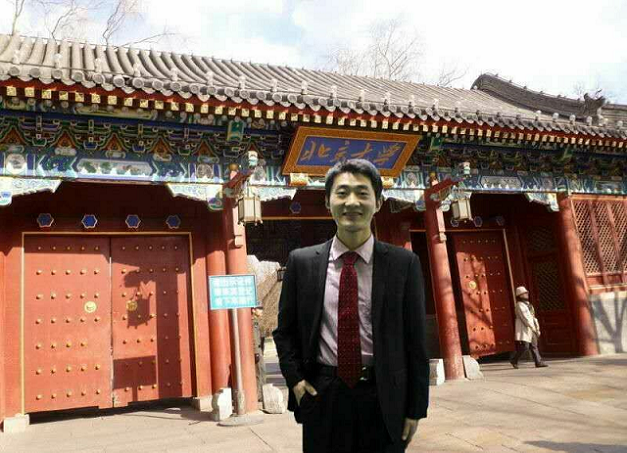
\includegraphics{shuwenhe.png}}
%写好一本书:工匠精神!用心打造!夜深写于北京大学图书馆。作者亲自一线带课,所带学生多人保送或考入清华北大,根据多年清华附中、101中学、人大附中、北大附中、十一学校,考试真题分析经验所得。用此书考上心目中名校学生无数!何书文北京大学硕士,资深数学名师、信息学竞赛算法名师,所带学生多名考入人大附中早培、清华附中优才、101 实验班、北大附中实验班等名校。全国中学数学联赛、全国中学数学竞赛的辅导老师,全国NOI、CSP信息学竞赛辅导名师。何书文老师在北京大学学习期间立志从事教育事业,帮学生授业解惑。何书文老师小学期间学习奥数,并多次获奖,为以后的学习与研究打下良好基础。何书文 老师在中学阶段数学、物理均获奖。何书文老师在小学中学期间一直为数学课代表,中小学大学期间担任班长,何书文老师在北京大学被选为科技一苑苑长,组织北大同学积极参与校各项活动,积极参与校学生会工作,何书文老师被北京大学评为优秀入党积极分子.何书文老师经常参加北京大学数学课题的研讨班。何书文 老师是北京大学数学系暑期学校全国选出40 名优秀中青年数学人才之一,参加伦敦国王学院、美国杜克大学、美国纽约大学、加拿大多伦多大学教授组成的学术研讨班,研究PDE(偏微分方程),量子力学方面的数学课题的研究工作,并获得优异成绩结业。何书文老师作为项目经理用数学建模方法给大型企业开发软件,用数学方法规划提高企业产能协作效率。何书文 老师致力于数学方面的教学与研究工作,所带多名孩子已经被点优才进入清华附中创新班,101 实验班,人大附中早培班,是家长值得信赖的老师。考上学生继续跟随何书文老师学习全国数学联赛,全国数学竞赛系列课程,同时学习NOI、IOI、ACM算法编程竞赛。
%%%%%%%%%%%%%%%%%%%%%%%%%%%%%%%%%%%%%%%%%%%%%%%%%%%%%%%%%%%%%%%%%%%%%%%%%%%%%%%%%%%%%%%%%%%%%%%%%%%%%%%%%%

%%%%%%%%%%%%%%%%%%%%%%%%%%%%%%%%%%%%%%%%%%%%%%%%%%%%%%%%%%%%%%%%%%%%%%%%%%%%%%%%%%%%%%%%%%%%%%%%%%%%%%%%%%
\title{Aliyun}
\maketitle
\tableofcontents % 显示目录
\newpage
\pagestyle{fancy}
%%%%%%%%%%%%%%%%%%%%%%%%%%%%%%%%%%%%%%%%%%%%%%%%%%%%%%%%%%%%%%%%%%%%%%%%%%%%%%%%%%%%%%%%%%%%%%%%%%%%%%%%%%

%\lhead{
\includegraphics{shuwenedu.png}}
%\rhead{科技特长生升学规划 何校长 电话微信15010729356}
%\lfoot{
\includegraphics{pku.png}算法第一人北大何书文}
%\rfoot{改变您家孩子命运的老师}
%%%%%%%%%%%%%%%%%%%%%%%%%%%%%%%%%%%%%%%%%%%%%%%%%%%%%%%%%%%%%%%%%%%%%%%%%%%%%%%%%%%%%%%%%%%%%%%%%%%%%%%%%%

%%%%%%%%%%%%%%%%%%%%%%%%%%%%%%%%%%%%%%%%%%%%%%%%%%%%%%%%%%%%%%%%%%%%%%%%%%%%%%%%%%%%%%%%%%%%%%%%%%%%%%%%%%
\chapter{ECS云服务器}
\url{https://ecs.console.aliyun.com/home#/}

\chapter{OSS对象存储}
\url{https://oss.console.aliyun.com/overview}\\
OSS Bucket:sidsa-statics 绑定的域名:sidsa-statics.sidsa.cn \\
OSS Bucket:sidsa-statics 绑定的域名:api-svc.sidsa.cn 上托管的 SSL证书\\
OSSBucket:sidsa-admin-ui 绑定的域名:admin.sidsa.cn 上托管的SSL证书

\section{Bucket列表}
\begin{tabular}{|c|c|c|c|}
\hline
Bucket名称 & 音标 & 译意 & 词根词缀\\
\hline
sidsa-admin-ui & /bre\textipa{I}s/ & n. 算法 & \\
\hline
sidsa-statics & /bre\textipa{I}s/ & n. 算法 & \\
\hline
\end{tabular}

\chapter{Kubernetes容器服务}
ACK容器服务\\
容器服务控制台\\
\url{https://cs.console.aliyun.com/#/k8s/cluster/list}\\
kubernetes ingress\\
集群类型\\
ASK标准版\\
连接信息\\
将以下内容复制到计算机\$HOME/.kube/config 文件下\\
\url{https://cs.console.aliyun.com/#/k8s/cluster/ccbdf99b67d43401ca4efa97df9c57ca1/v2/info/overview?clusterType=Ask&profile=Serverless&state=running&region=cn-beijing}

\section{安全组}
\url{https://ecs.console.aliyun.com/?spm=5176.2020520152.0.0.5b4716ddDZwSYN#/securityGroupDetail/region/cn-beijing/groupId/sg-2zeb7b92uw0gva2tum21/detail/intranetIngress}

\chapter{SLB负载均衡}
Server Load Balancer\\
负载均衡 SLB->传统型负载均衡 CLB/证书管理->替换证书

\chapter{DNS云解析}
\section{域名解析}
\url{https://dns.console.aliyun.com/?spm=5176.12818093_-128809398.0.dre2.225d16d0N6HJJQ#/dns/domainList}

\chapter{SSL数字证书管理服务}
\section{数字证书管理服务}
数字证书管理服务\\
\url{https://yundun.console.aliyun.com/?spm=5176.12818093_-1363046575.top-nav.87.3be916d05lDJYo&p=cas#/overview/cn-hangzhou}\\

\section{证书申请}
申请SSL证书出现审核失败的原因及处理方法\\
\url{https://help.aliyun.com/document_detail/48720.html?spm=0.2020520163.help.dexternal.6609p95bp95bWJ}\\
已经成功提交到CA公司,请您保持电话畅通,并及时查阅邮箱中来自CA公司的电子邮件。\\
三步完成DNS验证\\
1.登录域名管理控制台\\
2.在域名控制台添加DNS解析记录\\
\begin{tabular}{|c|c|}
\hline
配置项目 & 配置项值 \\
\hline
域名授权验证类型 & DNS \\
\hline
记录类型 & TXT \\
\hline
主机记录 & \_dnsauth \\
\hline
记录值 & 202307230000000dsvfzctvd42et8ujeg1ipeis8piq737hgz8j2968nue8uy97n \\
\hline
\end{tabular}


\section{设置TXT解析记录}
到域名服务商处设置\\
TXT记录不正确,删除旧的主机记录为\_dnsauth的TXT解析记录,并新添加\\
主机记录   \_dnsauth\\
记录值      202307230000000dsvfzctvd42et8ujeg1ipeis8piq737hgz8j2968nue8uy97n\\
删除之前所有的TXT解析记录

\section{SSL证书}
SSL证书\\
\url{https://yundun.console.aliyun.com/?spm=5176.12818093_-1363046575.top-nav.87.3be916d05lDJYo&p=cas#/certExtend/buy/cn-hangzhou}\\
阿里云配置ingress gateway ssl cert\\
\begin{tabular}{|c|c|c|c|}
\hline
 & 网关 & SSL & \\
\hline
ingress & gateway & ssl & cert\\
\hline
\end{tabular}

\section{ingress}
ALB Ingress配置HTTPS监听证书\\
\url{https://help.aliyun.com/zh/ack/ack-managed-and-ack-dedicated/user-guide/use-an-alb-ingress-to-configure-certificates-for-an-https-listener?spm=5176.smartservice_service_robot_chat_new.0.0.4d2df625AStz5j}\\
证书名称\\
alb-ingress-cert-v2 \\
证书域名\\
kubernetes ingress controller fake certificate\\
过期时间\\
2122年3月16日15:24:16\\
证书来源\\
用户上传

\section{上传SSL证书}
\url{https://help.aliyun.com/document_detail/98573.html?spm=0.2020520163.help.dexternal.529d1aYT1aYTTt#section-h2t-3mw-yfb}\\
\begin{tabular}{|c|c|c|c|}
\hline
PEM编码格式的SSL证书文件 & gateway & ssl & cert\\
\hline
\end{tabular}

\section{gateway}
\section{ssl}
\section{cert}

\chapter{VPC专有网络}
\url{https://vpc.console.aliyun.com/overview}\\


\clearpage
\end{document}
